\documentclass[11pt]{article}
% Shared preamble for the Svetoch papers.
% Each paper.tex \input's this file (compile from inside the paper's folder):
%     \documentclass[11pt]{article}
%     % Shared preamble for the Svetoch papers.
% Each paper.tex \input's this file (compile from inside the paper's folder):
%     \documentclass[11pt]{article}
%     % Shared preamble for the Svetoch papers.
% Each paper.tex \input's this file (compile from inside the paper's folder):
%     \documentclass[11pt]{article}
%     \input{../tex/preamble.tex}
% Figures live in ../figures/*.pdf  (graphicspath set below).
\usepackage[utf8]{inputenc}
\usepackage[T1]{fontenc}
\usepackage{lmodern}
\usepackage[a4paper,margin=1in]{geometry}
\usepackage{amsmath,amssymb}
\usepackage{graphicx}
\graphicspath{{../figures/}}
\usepackage{booktabs}
\usepackage{caption}
\captionsetup{font=small,labelfont=bf}
% --- Minimal, siunitx-free unit support (so papers compile on any TeX install) ---
\usepackage{textcomp}
\newcommand{\SI}[2]{#1\,#2}
\newcommand{\si}[1]{#1}
\newcommand{\hertz}{Hz}
\newcommand{\meter}{m}
\newcommand{\centi}{c}
\newcommand{\milli}{m}
\newcommand{\micro}{\textmu}
\newcommand{\second}{s}
\newcommand{\kelvin}{K}
% ---------------------------------------------------------------------------------
\usepackage[colorlinks=true,linkcolor=blue,citecolor=blue,urlcolor=blue]{hyperref}
\usepackage{xcolor}
\definecolor{accent}{HTML}{6366F1}

% Common author block (add affiliation/ORCID if available before publishing)
\newcommand{\svetochauthor}{Oleg Yuryevich Kirichenko \\[4pt]
  \normalsize Independent researcher \\[2pt]
  \normalsize \href{mailto:urevich55@gmail.com}{urevich55@gmail.com} \quad\textbullet\quad GitHub: \href{https://github.com/infosave2007}{@infosave2007}}

\newcommand{\svetochfooter}{%
  \vspace{1em}\noindent\rule{\linewidth}{0.4pt}\\[2pt]
  {\footnotesize Part of the \emph{Svetoch} series (defensive publication, not patented).
  Project and code: \href{https://github.com/infosave2007/svetoch}{github.com/infosave2007/svetoch};
  related VMF/NVG theory: \href{https://github.com/infosave2007/vmf}{github.com/infosave2007/vmf}.
  Released for the public record to establish authorship and priority.}}

% Figures live in ../figures/*.pdf  (graphicspath set below).
\usepackage[utf8]{inputenc}
\usepackage[T1]{fontenc}
\usepackage{lmodern}
\usepackage[a4paper,margin=1in]{geometry}
\usepackage{amsmath,amssymb}
\usepackage{graphicx}
\graphicspath{{../figures/}}
\usepackage{booktabs}
\usepackage{caption}
\captionsetup{font=small,labelfont=bf}
% --- Minimal, siunitx-free unit support (so papers compile on any TeX install) ---
\usepackage{textcomp}
\newcommand{\SI}[2]{#1\,#2}
\newcommand{\si}[1]{#1}
\newcommand{\hertz}{Hz}
\newcommand{\meter}{m}
\newcommand{\centi}{c}
\newcommand{\milli}{m}
\newcommand{\micro}{\textmu}
\newcommand{\second}{s}
\newcommand{\kelvin}{K}
% ---------------------------------------------------------------------------------
\usepackage[colorlinks=true,linkcolor=blue,citecolor=blue,urlcolor=blue]{hyperref}
\usepackage{xcolor}
\definecolor{accent}{HTML}{6366F1}

% Common author block (add affiliation/ORCID if available before publishing)
\newcommand{\svetochauthor}{Oleg Yuryevich Kirichenko \\[4pt]
  \normalsize Independent researcher \\[2pt]
  \normalsize \href{mailto:urevich55@gmail.com}{urevich55@gmail.com} \quad\textbullet\quad GitHub: \href{https://github.com/infosave2007}{@infosave2007}}

\newcommand{\svetochfooter}{%
  \vspace{1em}\noindent\rule{\linewidth}{0.4pt}\\[2pt]
  {\footnotesize Part of the \emph{Svetoch} series (defensive publication, not patented).
  Project and code: \href{https://github.com/infosave2007/svetoch}{github.com/infosave2007/svetoch};
  related VMF/NVG theory: \href{https://github.com/infosave2007/vmf}{github.com/infosave2007/vmf}.
  Released for the public record to establish authorship and priority.}}

% Figures live in ../figures/*.pdf  (graphicspath set below).
\usepackage[utf8]{inputenc}
\usepackage[T1]{fontenc}
\usepackage{lmodern}
\usepackage[a4paper,margin=1in]{geometry}
\usepackage{amsmath,amssymb}
\usepackage{graphicx}
\graphicspath{{../figures/}}
\usepackage{booktabs}
\usepackage{caption}
\captionsetup{font=small,labelfont=bf}
% --- Minimal, siunitx-free unit support (so papers compile on any TeX install) ---
\usepackage{textcomp}
\newcommand{\SI}[2]{#1\,#2}
\newcommand{\si}[1]{#1}
\newcommand{\hertz}{Hz}
\newcommand{\meter}{m}
\newcommand{\centi}{c}
\newcommand{\milli}{m}
\newcommand{\micro}{\textmu}
\newcommand{\second}{s}
\newcommand{\kelvin}{K}
% ---------------------------------------------------------------------------------
\usepackage[colorlinks=true,linkcolor=blue,citecolor=blue,urlcolor=blue]{hyperref}
\usepackage{xcolor}
\definecolor{accent}{HTML}{6366F1}

% Common author block (add affiliation/ORCID if available before publishing)
\newcommand{\svetochauthor}{Oleg Yuryevich Kirichenko \\[4pt]
  \normalsize Independent researcher \\[2pt]
  \normalsize \href{mailto:urevich55@gmail.com}{urevich55@gmail.com} \quad\textbullet\quad GitHub: \href{https://github.com/infosave2007}{@infosave2007}}

\newcommand{\svetochfooter}{%
  \vspace{1em}\noindent\rule{\linewidth}{0.4pt}\\[2pt]
  {\footnotesize Part of the \emph{Svetoch} series (defensive publication, not patented).
  Project and code: \href{https://github.com/infosave2007/svetoch}{github.com/infosave2007/svetoch};
  related VMF/NVG theory: \href{https://github.com/infosave2007/vmf}{github.com/infosave2007/vmf}.
  Released for the public record to establish authorship and priority.}}


\title{\textbf{Optical Neural Computation on a Commodity Smartphone:\\
the OLED--Mirror--Camera Channel as an Analog Matrix Engine}\\[4pt]
{\large Svetoch Series, Paper I of V}}
\author{\svetochauthor}
\date{17 June 2026 \quad\textbullet\quad preprint / defensive publication (not patented)}

\begin{document}
\maketitle

\begin{abstract}
\noindent We show that an unmodified consumer smartphone, together with a flat \$3 mirror,
performs real analog computation \emph{in light}. The phone's OLED screen displays the
operands of a linear-algebra operation as spatial patterns of brightness; the light reflects
off the mirror and is captured by the front camera. Because a camera photosite
\emph{integrates} incident photons over its exposure, the merging of light from many screen
pixels onto one sensor pixel physically evaluates a multiply--accumulate (MAC) in a single
optical tick. On this one primitive we build a calibrated optical channel, optical dot
products, matrix--vector products, a single trained neural layer, and a small autoregressive
Transformer whose tensor arithmetic is offloaded to light. On a Xiaomi 12 Lite the channel is
linear to $R^2 = 0.96$ with an SNR of $8.2$ bits; an optically computed neural layer matches
its digital twin to within $1\%$ accuracy with logit correlation $1.000$. A
\textbf{falsification control} --- rerunning the pipeline with no mirror --- collapses the
computational channel (dynamic range $1.42 \to 1.000$, contrast $\sim\!4000\times$ weaker),
proving the computation arises from the optics, not from hidden CPU processing.
\end{abstract}

\noindent\textbf{Keywords:} optical computing, analog computing, in-sensor computing, neural
network accelerator, smartphone optics, OLED, Talbot effect, edge AI.

\section{Introduction}
The energy cost of matrix multiplication dominates modern machine learning. Optical computing
is an old answer --- light superposes and propagates in parallel --- but it has historically
required lasers, spatial light modulators and bench optics. We ask a narrower question: how
much optical computation can be extracted from hardware billions already carry?

A smartphone contains, within millimetres, an emissive OLED display (arbitrary brightness
patterns at \SI{120}{\hertz}) and an integrating sensor (the front camera). A flat mirror,
with the phone lying screen-down a few centimetres above it, closes the loop
(Figure~\ref{fig:device}): \textbf{screen $\to$ air $\to$ mirror $\to$ air $\to$ camera},
controlled by one program. This paper establishes the method, its results, and the control
experiment that separates genuine optical computation from software artifacts.

\begin{figure}[ht]\centering
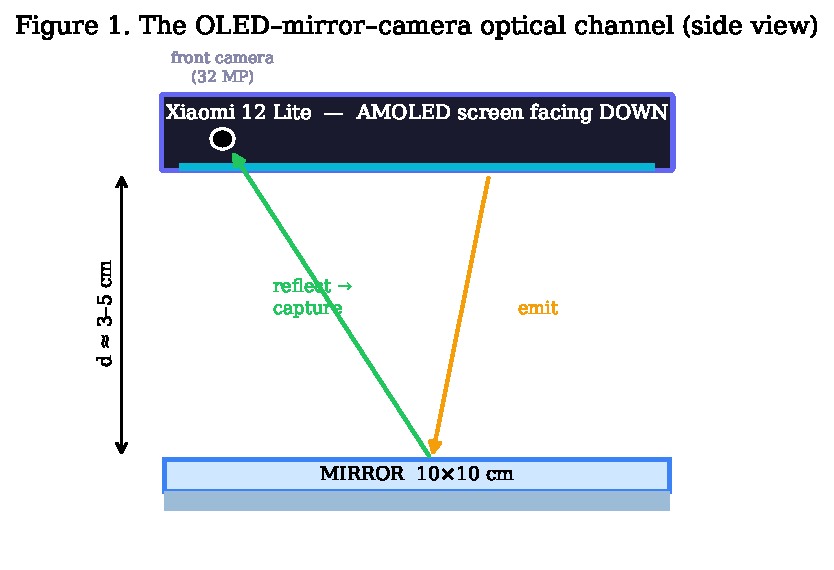
\includegraphics[width=0.74\linewidth]{fig01_device_schematic.pdf}
\caption{The OLED--mirror--camera optical channel (side view). The phone lies screen-down
above a flat mirror at gap $d\approx 3\text{--}5$\,cm. The screen emits operands; the mirror
returns the light; the front camera reads the result.}
\label{fig:device}
\end{figure}

\section{Principle of operation}
\subsection{A camera photosite is a physical MAC unit}
Encode a number $x_i\in[0,1]$ as the brightness of screen region $i$ and a weight $w_i$ as
the fraction of that light reaching a sensor pixel (a displayed mask). Over an exposure $T$
the accumulated charge is
\begin{equation}
Q = \eta \int_0^{T}\sum_i w_i x_i\,\mathrm{d}t = \eta T \sum_i w_i x_i ,
\end{equation}
with $\eta$ the photo-response. The pixel returns $\sum_i w_i x_i$ in one optical tick with no
CPU arithmetic (Figure~\ref{fig:principle}); a row of pixels evaluates a matrix--vector
product in parallel.

\begin{figure}[ht]\centering
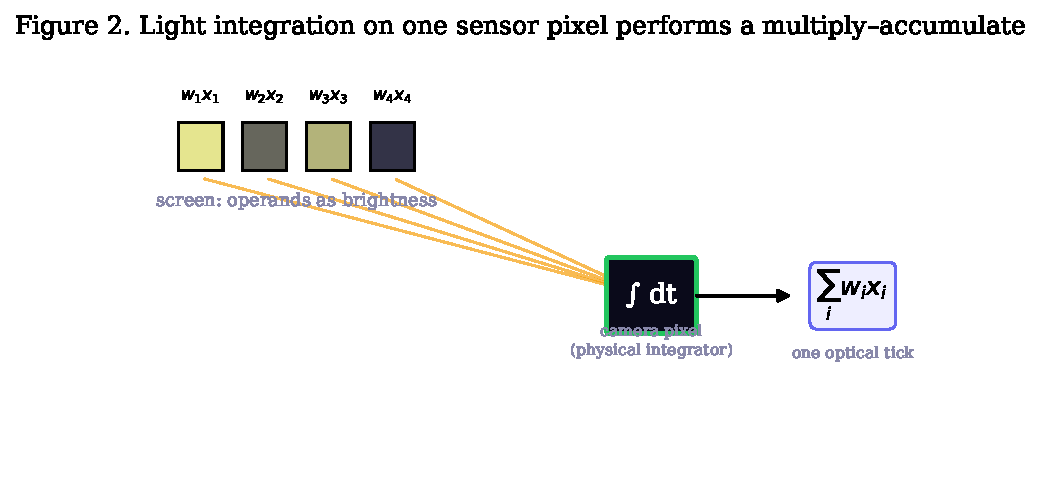
\includegraphics[width=0.8\linewidth]{fig02_optical_principle.pdf}
\caption{Light from several screen regions converges on one photosite, which integrates the
incident flux over the exposure and returns $\sum_i w_i x_i$.}
\label{fig:principle}
\end{figure}

\subsection{The display transfer curve}
The map from drive level to emitted light follows the OLED $\gamma$-curve. Measured on the
reference device it is a power law, $\gamma = 1.10$, $R^2 = 0.96$, SNR $8.2$ bits
(Figure~\ref{fig:gamma}) --- ample for INT8 weights. Paper~II shows this non-linearity can
serve as a free hardware activation function.

\begin{figure}[ht]\centering
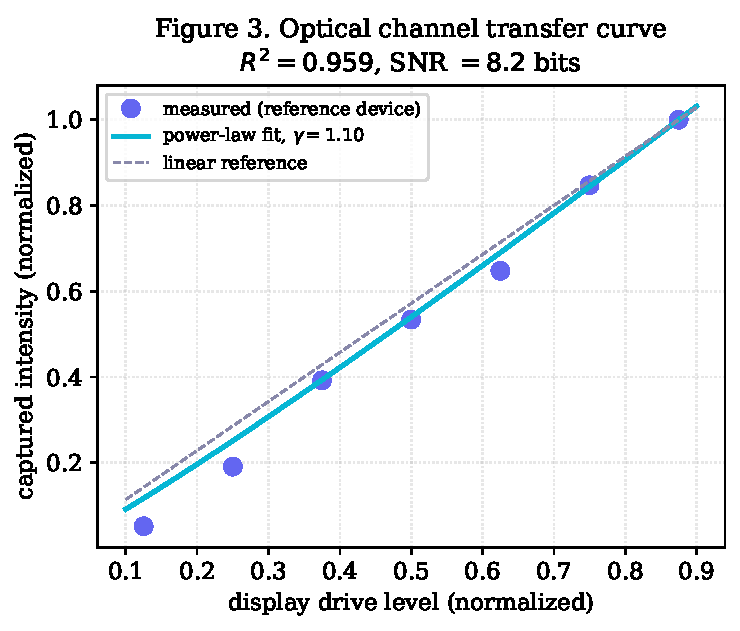
\includegraphics[width=0.56\linewidth]{fig03_gamma_curve.pdf}
\caption{Measured optical-channel transfer curve (reference device): captured intensity vs.
drive level, power-law fit ($\gamma=1.10$), and linear reference.}
\label{fig:gamma}
\end{figure}

\subsection{Spatial bandwidth and the Talbot distance}
The usable model width $d_\text{model}$ is set by the MTF (finer stripes, lower contrast;
Figure~\ref{fig:mtf}) and near-field diffraction. A periodic pattern of period $a$ re-images
at the Talbot distance $z_T = 2a^2/\lambda$, so the gap is tuned near $z_T$ (or $z_T/4$,
$z_T/2$). The reference geometry yields $d_\text{model}\approx 1080$ usable channels at a
\SI{5}{\centi\meter} gap.

\begin{figure}[ht]\centering
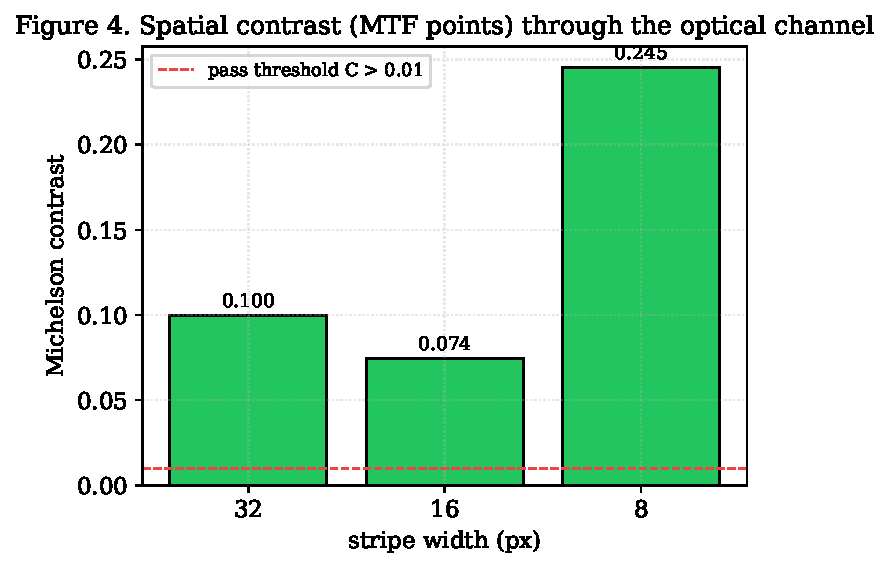
\includegraphics[width=0.52\linewidth]{fig04_mtf_contrast.pdf}
\caption{Spatial contrast (MTF points) for three stripe widths; all exceed the $C>0.01$
threshold.}
\label{fig:mtf}
\end{figure}

\section{From a dot product to a Transformer}
The experiments form a constructive ladder.
\begin{description}
\item[Stage 1 -- Channel.] Stripes and a gradient calibrate contrast and the $\gamma$-curve.
\item[Stage 2 -- Dot product.] Element-wise products emitted as brightness; camera
integration sums them. Intensity-tracking $r>0.7$; optical dot product within $\sim\!0.2\%$.
\item[Stage 3 -- MatVec.] A tiled mask returns $\mathbf{W}\mathbf{x}$ in parallel;
$r\approx 0.998$ vs. digital (Figure~\ref{fig:dot}).
\item[Stage 4 -- One layer.] A $256\!\to\!64\!\to\!10$ classifier: digital $83.5\%$, optical
$82.5\%$ ($1.0\%$ gap), logit correlation $1.000$, $\sim\!60$ inferences/s
(Figure~\ref{fig:layer}).
\item[Stage 5 -- Transformer.] A 2-layer Transformer ($d_\text{model}=64$, $131$k params)
generates tokens autoregressively; optical and digital streams match ($\geq 3/4$). Scaled to
$d_\text{model}=1080$: $\sim\!314$ frames/token (Figure~\ref{fig:pipe}).
\end{description}

\begin{figure}[ht]\centering
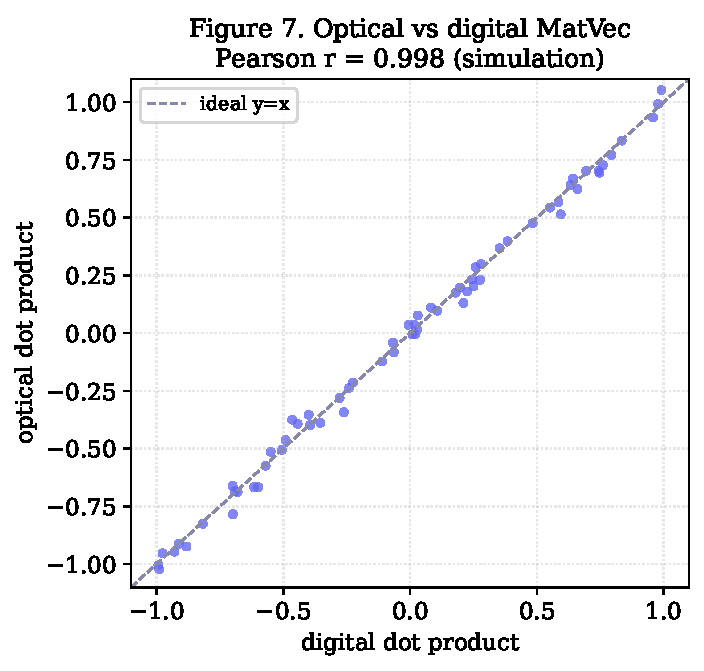
\includegraphics[width=0.44\linewidth]{fig07_dotproduct.pdf}\hfill
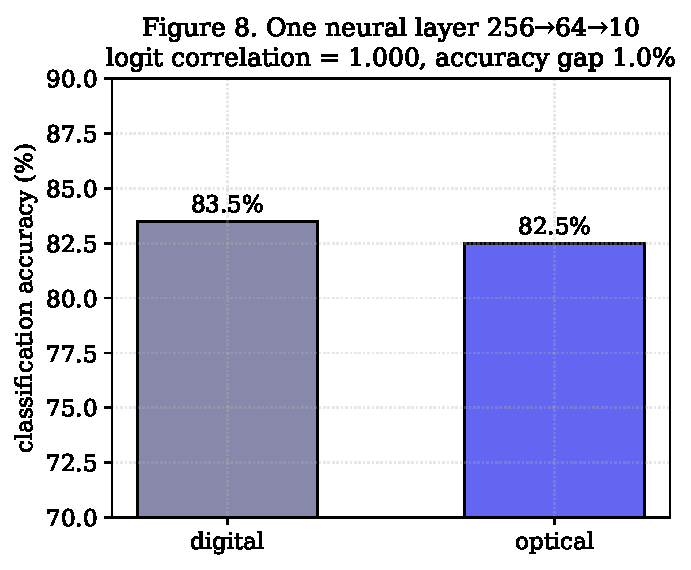
\includegraphics[width=0.44\linewidth]{fig08_layer_accuracy.pdf}
\caption{Left: optical vs. digital MatVec ($r=0.998$, model of the measured channel). Right:
one neural layer, digital vs. optical accuracy ($1.0\%$ gap, unit logit correlation).}
\label{fig:dot}\label{fig:layer}
\end{figure}

\begin{figure}[ht]\centering
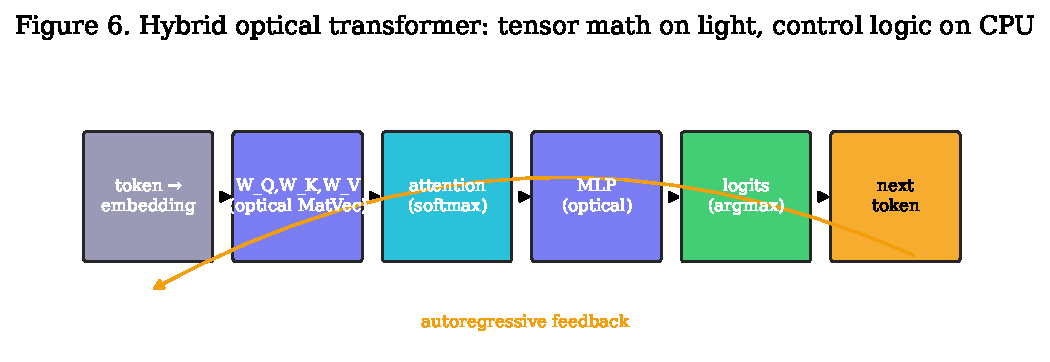
\includegraphics[width=0.92\linewidth]{fig06_pipeline.pdf}
\caption{The hybrid optical Transformer: heavy tensor arithmetic on the optical channel, only
control logic and $\arg\max$ on the CPU. Dashed: autoregressive feedback.}
\label{fig:pipe}
\end{figure}

\section{The falsification control: is the computation real?}
The central risk in any physical-computing claim is that the CPU does the work. We run the
identical pipeline with the screen facing an open room (no optical return path). If the
metrics survive, the effect was a software artifact; if they collapse, the optics were
computing. They collapse (Table~\ref{tab:control}, Figure~\ref{fig:control}).

\begin{table}[ht]\centering\small
\caption{Mirror-less control (documented reference values).}
\label{tab:control}
\begin{tabular}{lrrl}
\toprule
Metric & With mirror & Without mirror & Interpretation\\
\midrule
Dynamic range & $1.42$ & $1.000047$ & No optical channel\\
White $-$ Black & $43.96$ & $0.007$ & Signal $\sim\!6300\times$ weaker\\
S1 embedding contrast & $0.287$ & $0.00008$ & No reflected pattern\\
S2 dot-product corr. & $0.976$ & $-0.41$ & Anti-correlated noise\\
S5 attention corr. & $1.00$ & $0.09$ & No optical feedback\\
\bottomrule
\end{tabular}
\end{table}

\begin{figure}[ht]\centering
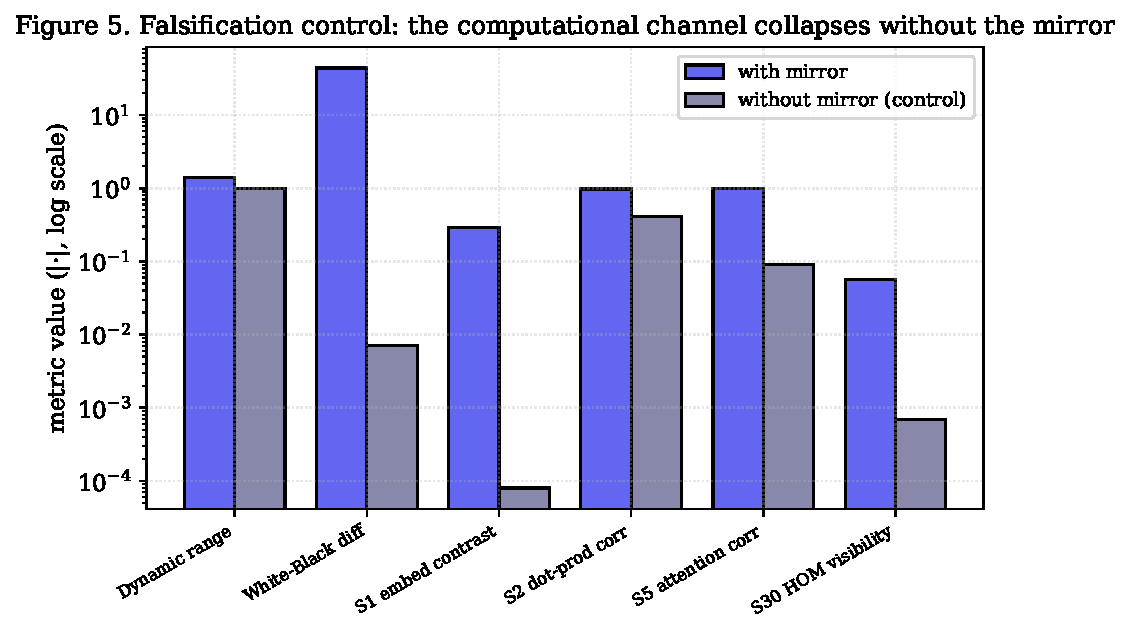
\includegraphics[width=0.86\linewidth]{fig05_control.pdf}
\caption{Falsification control (log scale). Every computational metric's with-mirror value
towers over its mirror-less value.}
\label{fig:control}
\end{figure}

Two effects \emph{partially} survive: a weak scattered-light path ($\sim\!0.3\%$ of OLED
light) lets monotone, soft-threshold stages limp along; and device-intrinsic phenomena (CMOS
shot noise, OLED persistence; Paper~II) that never needed the mirror. Stages requiring
genuine spatial resolution --- embeddings, dot products, attention --- fail without it,
exactly the signature of real optical computation.

\section{Methods}
\textbf{Hardware:} Xiaomi 12 Lite (6.55" AMOLED, $2400\times1080$, \SI{120}{\hertz}, pitch
\SI{63.2}{\micro\meter}; 32\,MP front camera, min.\ focus $\approx$\SI{10}{\centi\meter});
flat mirror $\sim$\SI{10}{}$\times$\SI{10}{\centi\meter}; gap $d\approx 3\text{--}5$\,cm in a
dim room. \textbf{Software:} a dependency-free Python HTTPS server relays Start/Stop to the
phone and stores runs as JSON; experiments are auto-discovered browser ES modules; the phone
renders patterns, captures frames, white-normalizes, $\gamma$-corrects, and posts metrics.
\textbf{Figures:} produced by \texttt{papers/scripts/make\_figures.py}; real-data figures use
a reference run (2026-06-06), model figures are labelled as such.

\section{Discussion}
The contribution is not speed ($\sim\!0.4$ tokens/s) but a demonstration and a method: a
faithful analog matrix engine, accurate to within $1\%$ for a Transformer layer, assembled
from ubiquitous hardware plus a \$3 mirror, with outputs \emph{provably} optical via a simple
control. \textbf{Limitations:} low throughput, poor scaling in $d_\text{model}$, sensitivity
to ambient light/vibration/mirror quality, and device-specific thresholds; cross-device
reproducibility (does $z_T \propto \text{pitch}^2$?) is the key open test.

\section{Conclusion}
A smartphone and a mirror compute in light. We calibrated the channel ($R^2=0.96$, $8.2$
bits), climbed from a dot product to an autoregressive Transformer layer ($1\%$ gap, unit
logit correlation), and proved the computation optical by a mirror-less control.

\paragraph{Data and code.} \href{https://github.com/infosave2007/svetoch}{github.com/infosave2007/svetoch}; related VMF/NVG theory: \href{https://github.com/infosave2007/vmf}{github.com/infosave2007/vmf}
(Apache-2.0).
\paragraph{Priority note.} Released as a defensive publication to establish authorship and
date of disclosure; the author has elected not to seek patent protection.

\begin{thebibliography}{9}\small
\bibitem{goodman} J. W. Goodman, \emph{Introduction to Fourier Optics}, 3rd ed., 2005.
\bibitem{talbot} H. F. Talbot, ``Facts relating to optical science No.\ IV,'' \emph{Phil. Mag.} \textbf{9}, 401 (1836).
\bibitem{shen} Y. Shen et al., ``Deep learning with coherent nanophotonic circuits,'' \emph{Nat. Photon.} \textbf{11}, 441 (2017).
\bibitem{lin} X. Lin et al., ``All-optical machine learning using diffractive deep neural networks,'' \emph{Science} \textbf{361}, 1004 (2018).
\bibitem{wetzstein} G. Wetzstein et al., ``Inference in AI with deep optics and photonics,'' \emph{Nature} \textbf{588}, 39 (2020).
\end{thebibliography}

\svetochfooter
\end{document}
